\section{Episode 59: Listing Heavily}

\medskip

\DndDropCapLine{T}he gang, relaxing after a stressful afternoon, sit around Myron’s list, and between Anthony, the bookburner’s library and Riphard actually paying attention (so that he can carry on ignoring his children) they actually end up doing quite well, filling out a lot of the gaps.\medskip

Myron reluctantly says that he thinks the only way they’re going to survive is if they get The People on their side, track down everyone they can that might be able to help them, and that they might need to be… heroes...\medskip

In the middle of his awkward speech, Burnie walks downstairs and starts talking to Myron about his birdson, despite the fact that Myron is upstairs trying to do a speech. He removes the poisoned crossbow bolt from his buttocks, glowing with pride, and places it in a crack in the wall.\medskip

Myron comes downstairs, and asks Burnie what he’s up to, and why he walked out of his awkward speech.\medskip

Together, they try and work out who to talk to next. They decide to see if they can find Rolltop Kandian. Rip asks if they can go via checking in with Derek Bobacious.\medskip

Riphard talks to Derek by himself first, to try and get some dirt on Anthony, and drive a wedge between Northern Rock PLC and The Guild of Coin. Derek seems to like Anthony for some reason.\medskip

Everyone else comes in and everyone chats about business and all that sort of boring shit.\medskip

On the way out, they check to see in Rolltop Kandian is still in the police force, apparently, he’s got a big promotion, and everything, so, they head across to see him.\medskip

They get shown up to his office, where the overworked, salt of the earth, police chief, sits behind a big pile of papers. Him and Myron reminisce about old times for a bit, and then get down to business, talking about any potential changes in the church’s relationship to the city (there are none) and any more information he might have about the people on the list (there is some).\medskip

The SRA are in Golding’s Bay, apparently, blowing up the infrastructure servicing, apparently, and Vuthelle is trying to rebuild her sunken isle.\medskip

He mentions that he’d love to be more helpful, but there seems to be some sort of serial killer on the loose.\medskip

On the way out, Myron arranges to go for a drink after Rolltop finishes.\medskip

Just as they leave, Rip tries to get dirt on Anthony from the policeman too.\medskip

As evening draws in, Myron heads off to meet up with Rolltop. Burnie hides inexpertly behind a pot plant, trying to follow and eavesdrop, Myron tells him to fuck off and let him meet his old friend in peace, and Burnie slithers off down a manhole cover somewhere.\medskip

Myron gets to the bar a few hours early, and is sitting there looking uneasy when Rolltop gets there. He tells him that the murderer is a goblin living in the sewers, but that he’s very dangerous and he shouldn’t send his men in to find him if he doesn’t want to lose them. Then he runs out leaving his drinks undrunk, and Rolltop asking him how he knows.\medskip

Burnie has found the printing press Lillith gave them the keys for, hidden in the sewers, and makes a note of how to get there from the fire house.\medskip

Burnie then goes to the Guild of Assassins, to try and track down Estebaun, who, last he knew, went back there after the Bookburners got broken up. He walks up to the front door, and asks the shadowy figure behind the hatch if he can talk to Estebaun. Not entirely surprisingly, they aren’t too keen on telling randoms who is and isn’t an assassin, even in this town.\medskip

Burnie, in a moment of uncharacteristic brilliance, asks if he could hire an assassin called Estebaun to assassinate an ant on the ground. He is given a price of 50 gold, which he pays through a slot in the door, once he gets it to accept his coin. He scoops up the ant into a glass jar and waits in an alley.\medskip

Meanwhile, across the city, Myron decides to go and check in with the Garys, who have apparently set themselves up over the other side of town.\medskip

Back in the alley, after about 40 minutes has passed, a sickly-looking young assassin gets booted out of the door, and comes over to kill the ant. Unfortunately, by now, Burnie has named the thing and his rampant paternal instinct has latched onto it.\medskip

Through a bit of bribery and a bit of manipulation he tries to convince the assassin to kill the ant using the time-honoured method of taking care of it until it dies. Burnie is assured that this will happen, in a way that convinces only Burnie.\medskip

Estebaun is apparently still around, and now works as an instructor for the newer recruits. Burnie also tells this kid to check on his son at some point, and also that his name is Tim, which ends up actually being right, despite how much the kid tried not to tell him.\medskip

On the other side of town, Myron has got to the Garys. Rip is with him, but he hasn’t realised yet.\medskip

The Garys seem to have turned a corner. After nearly dying of a chicken disease, and seeing Gary in a vision, they now operate as a pseudo-religious movement, espousing peace and protection, with Abigail - no longer crazy, now slightly Scouse - at the head.\medskip

They talk to her, and it comes out in conversation that Rip knew Gary first hand. Sensing opportunity, Rip and Myron tell Abigail what Gary was fighting for, for the 8, for the future, for the souls of everyone alive today. The Garys sign up to fight the good fight. They are offered use of the printing press once its up and running, and only ask that they be allowed to carry on being peaceful.\medskip

Returning to the firehouse, the gang try and decide what to do next. They decide to head across to New Abbergast, and then swing by Golding’s Bay on the way back. They all set about making preparations to head out again, none so more enthusiastically than Riphard.\medskip

\textbf{EPILOGUE}\medskip

A smoke filled office, late at night. Everyone else has gone home, but Rolltop Kandian sits in his office alone, staring at a pile of evidence laid out on his desk, illuminated by the shafts of pale white light that shine in through his blinds from the moon outside.\medskip

If what the gnome says is right, then there’s not many grey areas left in this case, not many links left to make. These murders seem to all be fitting together, and the patterns growing more obvious. The hiding places are shrinking rapidly.\medskip

Such a shame. This case had served him so well. Still, he could probably get away with a few more, but he’d have to move quick. He’d have to be more careful now, though.\medskip

r/https://www.youtube.com/watch?v=AIPGyKGuWeA

\vspace*{5mm}

\begin{center}
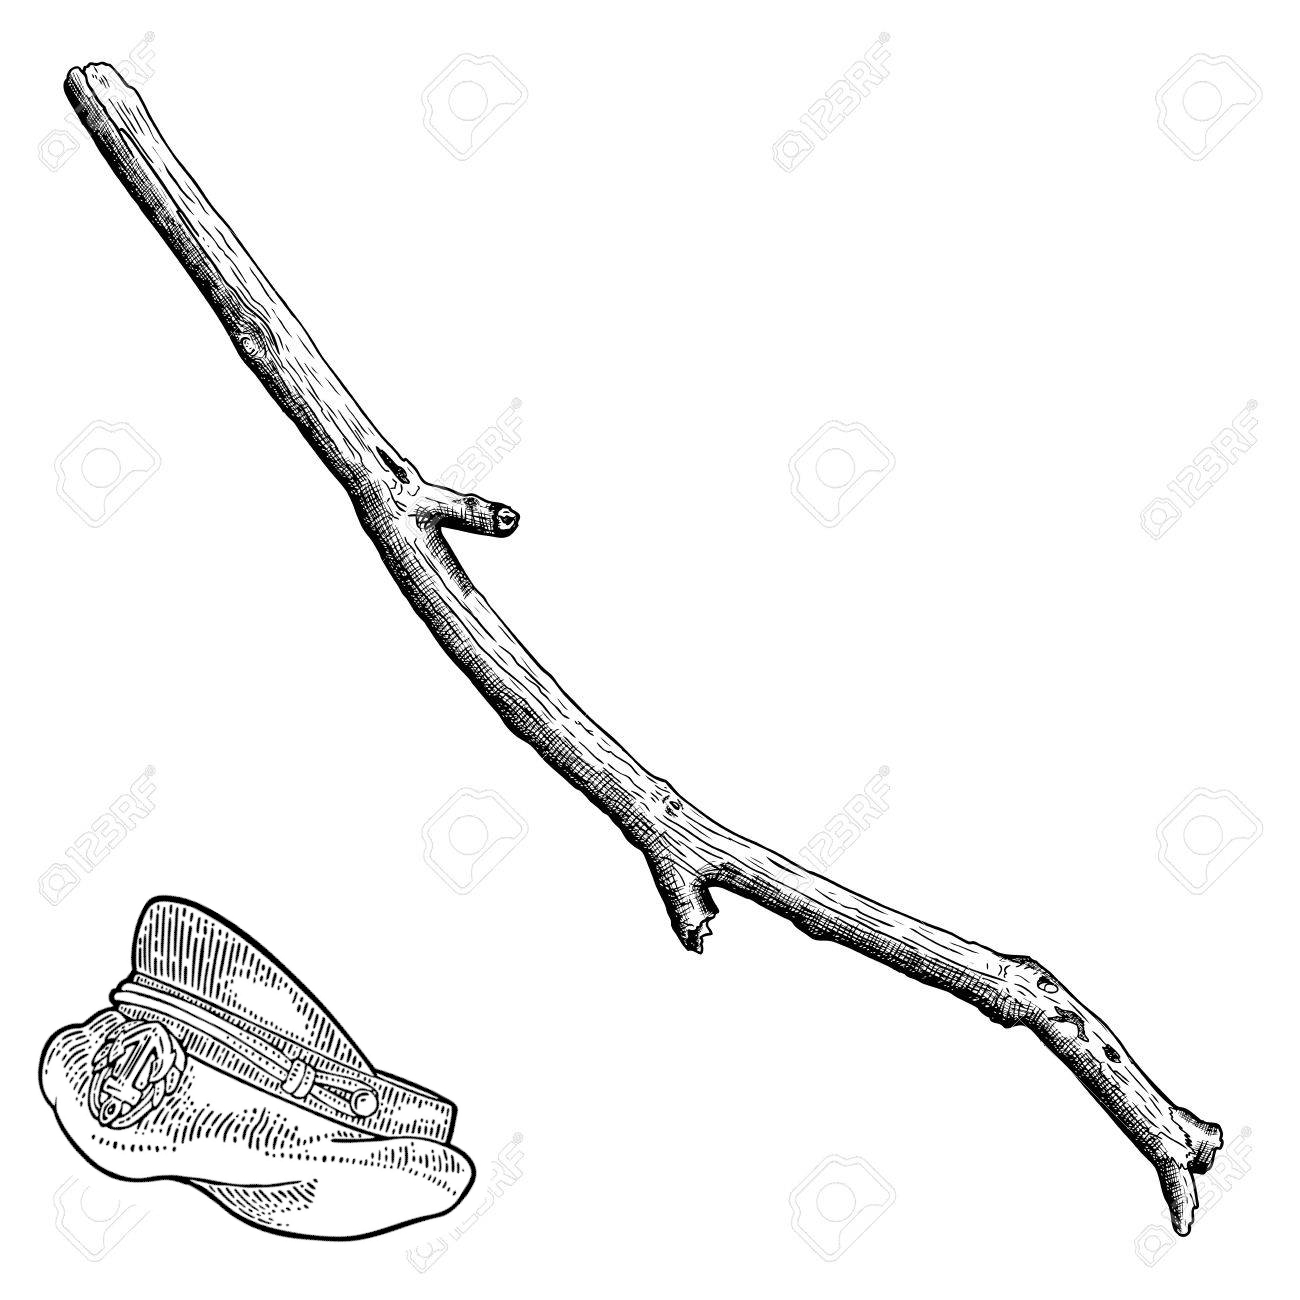
\includegraphics[width=\textwidth]{./content/img/xxx.jpg}
\begin{figure}[h]
\end{figure}
\end{center}

\clearpage
